\documentclass[10pt, letterpaper]{report}
% !TeX program = xelatex
%==================PREAMBOLO=======================%
\usepackage[utf8]{inputenc}
\usepackage{psvectorian}
\usepackage{pgfplots}
\usepackage[Rejne]{fncychap}
\usepackage[export]{adjustbox}
\usepackage[T1]{fontenc}
\usepackage{lmodern}
\usepackage{blindtext}
\usepackage{pdfpages}
\usepackage[shortlabels]{enumitem}
\usepackage{moresize}
\usepackage{graphicx} % Required for inserting images
\usepackage{hyperref}
\usepackage{listings}
\usepackage[table,xcdraw]{xcolor}
\usepackage{amssymb}
\usepackage{amsmath}
\usepackage[english]{babel}
\usepackage{nicefrac, xfrac}
\usepackage{tikz}
\usepackage{tikz-3dplot}
\usepackage{tikz-cd}
\usepackage{mathrsfs} 
\usepackage{titletoc}
\usepackage{fancyhdr}
\usepackage{psvectorian,lipsum}
\usepackage{fourier-orns}
\usepackage{lipsum}
\usepackage{wrapfig}
\usepackage{multicol}
\usepackage[paper=a4paper,left=25mm,right=25mm,bottom=25mm,top=25mm]{geometry}
\definecolor{light-gray}{gray}{0.95}
\definecolor{cop}{HTML}{f7ecd7}
\definecolor{copAut}{HTML}{ababab}
\definecolor{copAut2}{HTML}{c3c3e6}
\definecolor{purcop}{HTML}{d0d3db}
\definecolor{sapienza}{HTML}{660f1d}
\definecolor{lightSapienza}{HTML}{e3d3d5}
\definecolor{darkgreen}{HTML}{008000}
\definecolor{cartaRiciclata}{HTML}{fcfcf7}
\newcommand{\redText}[1]{\color{red}#1\color{black}}
\newcommand{\code}[1]{\colorbox{light-gray}{\texttt{#1}}}
\newcommand{\codee}[1]{\colorbox{white}{\texttt{#1}}}
\newcommand{\K}{{\mathbb K}}
\newcommand{\notimplies}{%
  \mathrel{{\ooalign{\hidewidth$\not\phantom{=}$\hidewidth\cr$\implies$}}}}
\newcommand{\flowerLine}{ \begin{center}\decofourleft\hphantom{ }\decoone\hphantom{ }\decofourright\hphantom{}\hphantom{aa}
\decofourleft\hphantom{ }\decoone\hphantom{ }\decofourright\hphantom{}\hphantom{aa}
\decofourleft\hphantom{ }\decoone\hphantom{ }\decofourright\hphantom{}\hphantom{aa}
\decofourleft\hphantom{ }\decoone\hphantom{ }\decofourright\hphantom{}\hphantom{aa} 
\decofourleft\hphantom{ }\decoone\hphantom{ }\decofourright\hphantom{}\hphantom{aa}
\decofourleft\hphantom{ }\decoone\hphantom{ }\decofourright\hphantom{}\hphantom{aa}
\decofourleft\hphantom{ }\decoone\hphantom{ }\decofourright\hphantom{}\hphantom{aa}
\decofourleft\hphantom{ }\decoone\hphantom{ }\decofourright\hphantom{}\hphantom{aa}
\decofourleft\hphantom{ }\decoone\hphantom{ }\decofourright\hphantom{}\hphantom{aa}
\end{center}}
\definecolor{g}{RGB}{60, 50, 50}
\newcommand{\textg}[1]{\color{g}{\textbf{#1}}\color{black}}
\newcommand{\teo}[1]{{\large\color{sapienza}\textbf{Teorema #1 :\hphantom{a}}}}
\newcommand{\defi}[1]{{\large\color{sapienza}\textbf{Definizione #1 :\hphantom{a}}}}
\newcommand{\claim}[1]{{\color{sapienza}\textbf{Claim #1 :\hphantom{a}}}}
\newcommand{\lemma}[1]{{\color{sapienza}\textbf{Lemma #1 :\hphantom{a}}}}
\newcommand{\dimo}[1]{{\color{sapienza}\textbf{Dimostrazione #1 :\hphantom{a}}}}
\newcommand{\prop}[1]{{\color{sapienza}\textbf{Proposizione #1 :\hphantom{a}}}}
\newcommand\greybox[1]{%
  \vskip\baselineskip%
  \par\noindent\colorbox{light-gray}{%
    \begin{minipage}{\textwidth}#1\end{minipage}%
  }%
  \vskip\baselineskip%
}
\newcommand\sapbox[1]{%
  \vskip\baselineskip%
  \par\noindent\colorbox{lightSapienza}{%
    \begin{minipage}{\textwidth}#1\end{minipage}%
  }%
  \vskip\baselineskip%
}
\newcommand{\ridFunc}{{f:\Sigma^*\rightarrow \Sigma^*}}
\newcommand{\rid}{{\le_m^P}}
\newcommand{\Z}{{\mathbb Z}}
\newcommand{\blank}{{\sqcup}}
\newcommand{\Prob}{{\mathbb P}}
\newcommand{\R}{{\mathbb R}}
\newcommand{\VA}{{\mathbb E}}
\newcommand{\N}{{\mathbb N}}
\newcommand{\quat}{{\mathbb H}}
\newcommand{\C}{{\mathbb C}}
\newcommand{\Sn}{{\mathcal S_n}}
\newcommand{\An}{{\mathcal A_n}}
\newcommand{\E}{{\mathcal E}}
\newcommand{\B}{{\mathcal B}}
\newcommand{\mcm}{{\text{mcm}}}
\newcommand{\rg}{{\text{rg}}}
\newcommand{\ve}{{\bar v}}
\newcommand{\spaz}{{\text{\hphantom{aa}}}}
\newcommand{\MCD}{{\text{MCD}}}
\newcommand{\tc}{{\text{ tale che }}}
\newcommand{\supp}{{\text{Supp}}}
\newcommand{\acc}{\\\hphantom{}\\}
\newcommand{\esempio}[1]{{\acc\large\color{sapienza}\textbf{Esempio #1 \hphantom{a}}\acc}}
\newcommand{\bra}[1]{\langle #1 \rangle}
\newcommand{\aut}{{\text{Aut}}}
\newcommand{\Span}{{\text{Span}}}
\newcommand{\End}{{\text{End}}}
\newcommand{\cen}{{\text{Centro}}}
\newcommand{\norm}{{\unlhd}}
\newcommand{\ciclS}{{\left \langle }}
\newcommand{\ciclE}{{\right \rangle }}
\newcommand{\boxedMath}[1]{\begin{tabular}{|c|}\hline \texttt{#1} \\ \hline\end{tabular} :} 
\newcommand{\shell}[1]{\colorbox{black}{\textcolor{white}{\texttt{#1}}}}
\newcommand{\eqImportante}[1]{\begin{center}\huge\lefthand\hphantom{a}
    \normalsize\texttt{#1}
    \hphantom{aaa}\huge\righthand\end{center}}

\fancyhf{}
\pagestyle{fancy}
\usepackage{pgf-pie}  
\usetikzlibrary{positioning}

\renewcommand{\headrule}{%
\vspace{-8pt}\hrulefill
\raisebox{-2.1pt}{\quad\decothreeleft\decotwo\decothreeright\quad}\hrulefill}

%sta roba serve per il codice C
\definecolor{mGreen}{rgb}{0,0.6,0}
\definecolor{mGray}{rgb}{0.5,0.5,0.5}
\definecolor{mPurple}{rgb}{0.58,0,0.82}
\definecolor{backgroundColour}{rgb}{0.95,0.95,0.92}

\lstdefinestyle{CStyle}{
    backgroundcolor=\color{backgroundColour},   
    commentstyle=\color{mGreen},
    keywordstyle=\color{magenta},
    numberstyle=\tiny\color{mGray},
    stringstyle=\color{mPurple},
    basicstyle=\footnotesize,
    breakatwhitespace=false,         
    breaklines=true,                 
    captionpos=b,                    
    keepspaces=true,                 
    numbers=left,                    
    numbersep=5pt,                  
    showspaces=false,                
    showstringspaces=false,
    showtabs=false,                  
    tabsize=2,
    language=C
}
\lstdefinestyle{CppStyle}{
    backgroundcolor=\color{backgroundColour},   
    commentstyle=\color{mGreen}\ttfamily,
    morecomment=[l][\color{magenta}]{\#}
    keywordstyle=\color{blue}\ttfamily,
    numberstyle=\tiny\color{mGray},
    stringstyle=\color{red}\ttfamily,
    basicstyle=\ttfamily,
    breakatwhitespace=false,         
    breaklines=true,                 
    captionpos=b,                    
    keepspaces=true,                 
    numbers=left,                    
    numbersep=5pt,                  
    showspaces=false,                
    showstringspaces=false,
    showtabs=false,                  
    tabsize=2,
    language=C
}
\lstset{language=C++,
                basicstyle=\ttfamily,
                keywordstyle=\color{blue}\ttfamily,
                stringstyle=\color{red}\ttfamily,
                commentstyle=\color{green}\ttfamily,
                morecomment=[l][\color{magenta}]{\#}
}
%fine roba che serve per il codice C
\usepackage{minted}
\usepackage{algorithm}
\usepackage{algpseudocode}
\newcommand{\titolo}{Artificial intelligence }

 %TOGLI COMMENTO SE USI XELATEX
%\usepackage{fontspec}
\title{\titolo} %========TITOLO========%
\author{Marco Casu}
\date{\vspace{-5ex}}
\begin{document}

%==================COPERTINA=======================%
\begin{titlepage}
    
\begin{center}
    %TOGLI COMMENTO SE USI XELATEX
   %\setmainfont{Palace Script MT}
   \HUGE Marco Casu\acc
\end{center}
\thispagestyle{empty}
\begin{figure}[h]
    \centering{
        %l'immagine deve avere una risoluzione 2048x2048
        
\includegraphics[width=1\textwidth ]{images/Copertina.png}
    }
\end{figure}
\vfill 
\centering 
\includegraphics[width=0.4\textwidth ]{../../preamble/Stemma_sapienza.png} \acc
\centering \Large \color{sapienza}Faculty of Information Engineering, Computer Science and Statistics\\
Department of Computer, Control and Management Engineering\\
Master's degree in Artificial Intelligence and Robotics
\end{titlepage}

%===================FINE COPERTINA======================%
\newpage
%\pagecolor{cartaRiciclata}%\setmainfont{Algerian}
\Large
This document summarizes and presents the topics for the \titolo course for the Master's degree in Artificial Intelligence and Robotics at Sapienza University of Rome. The document is free for any use. If the reader notices any typos, they are kindly requested to report them to the author.
\vfill
\begin{figure}[h!]
    \raggedright
    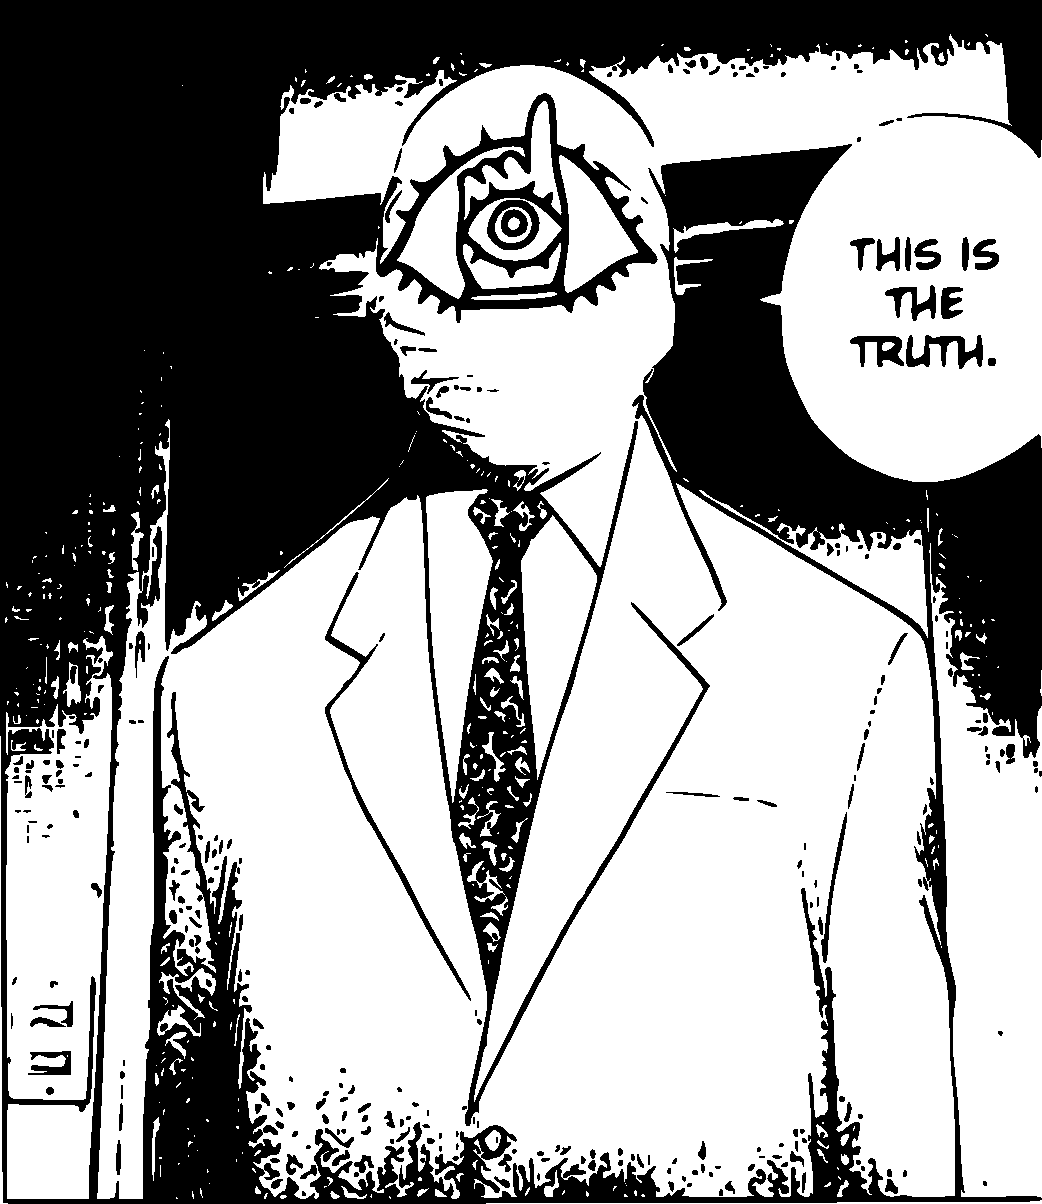
\includegraphics[width=0.4\textwidth,right ]{../../preamble/tomodachi.pdf} 
\end{figure}
\newpage %\setmainfont{Times New Roman}
\normalsize

\tableofcontents 
\newpage

%==================FOOTER e HEADER=======================%
\fancyhf{}
\fancyhead[L]{\nouppercase{\leftmark}}
\fancyhead[R]{Sezione \thesection}
\fancyfoot[C]{\thepage}
\fancyfoot[L]{\titolo}
\fancyfoot[R]{ Marco Casu}
%\fancyfoot[R]{\setmainfont{Palace Script MT}\huge Marco Casu \setmainfont{Times New Roman}}
%==================FOOTER e HEADER=======================%
\newtheorem{definition}{Definition}
\newtheorem{theorem}{Theorem}
%==================INIZIO======================%
\chapter{Introduzione}
\section{Basic Definitions}
In the context of the artificial intelligence, an \textbf{agent} is an entity that can\begin{itemize}
    \item Perceive the environment through \textit{sensors} (percepts)
    \item Act upon the environment through \textit{actuators} (actions).
\end{itemize}
We say that an agent is \textbf{rational} if he selects the action that maximize a given \textit{performance measure}, informally, he attempts to do ''the right thing''. The best case is hypothetical and often unattainable, because the agent usually can't perform all the actions needed, and can't perceive all the information about the environment.\bigskip

An agent has a performance measure $M$ and a set $A$ of all possible actions, given percept a sequence $A$ and knowledge $K$ (data), he has to select the next action $a\in A$, is a map\begin{equation}
    M\times P\times K \longrightarrow A.
\end{equation} 
An action $a$ is optimal if it maximize the expected value of $M$, given the sequence $P$ and the knowledge $K$. An agent is rational if he always chooses the optimal action. More specifically, an agent consists in two components:\begin{itemize}
    \item an architecture which provides an interface to the environment
    \item a program executed on that architecture.
\end{itemize}
There are some limitation that we aren't considering, such as the fact that determining the optimal choice could take too much time or memory on the architecture.

\subsection{Types of Agents}
There are different kinds of agents, a \textbf{Table Driven Agent} is the simplest form of agent architecture. It's essentially a look-up table that maps every possible sequence of percepts (what the agent has sensed so far) to a corresponding action the agent should take. His behavior can be resumed in the algorithm \ref{alg:table_agent}.

\begin{algorithm}
    \caption{Table Driven Agent}\label{alg:table_agent}
    \begin{algorithmic}
    \Require \textit{percepts}
    \State \textbf{persistent}: \textit{percepts}, a sequence, initially empty
    \State\hphantom{persistent: .} \textit{table}, a table of actions, indexed by percept sequences, initially fully specified
    \State append \textit{percept} to the end of \textit{percepts} 
    \State \textit{action}$\leftarrow$\texttt{LookUp}(\textit{percepts,table})
    \State\Return \textit{action}
    \end{algorithmic}
\end{algorithm}
\bigskip


A \textbf{Reflex Agent} consists in three components:\begin{itemize}
    \item sensors to get information from the environment
    \item a decision making process, in form of a \textit{condition-action rules}, typically looks like \texttt{IF (condition) THEN (action)}.
    \item actuators, the outputs that allow the agent to affect or change the environment.
\end{itemize}

\begin{figure}[h!]
    \centering
    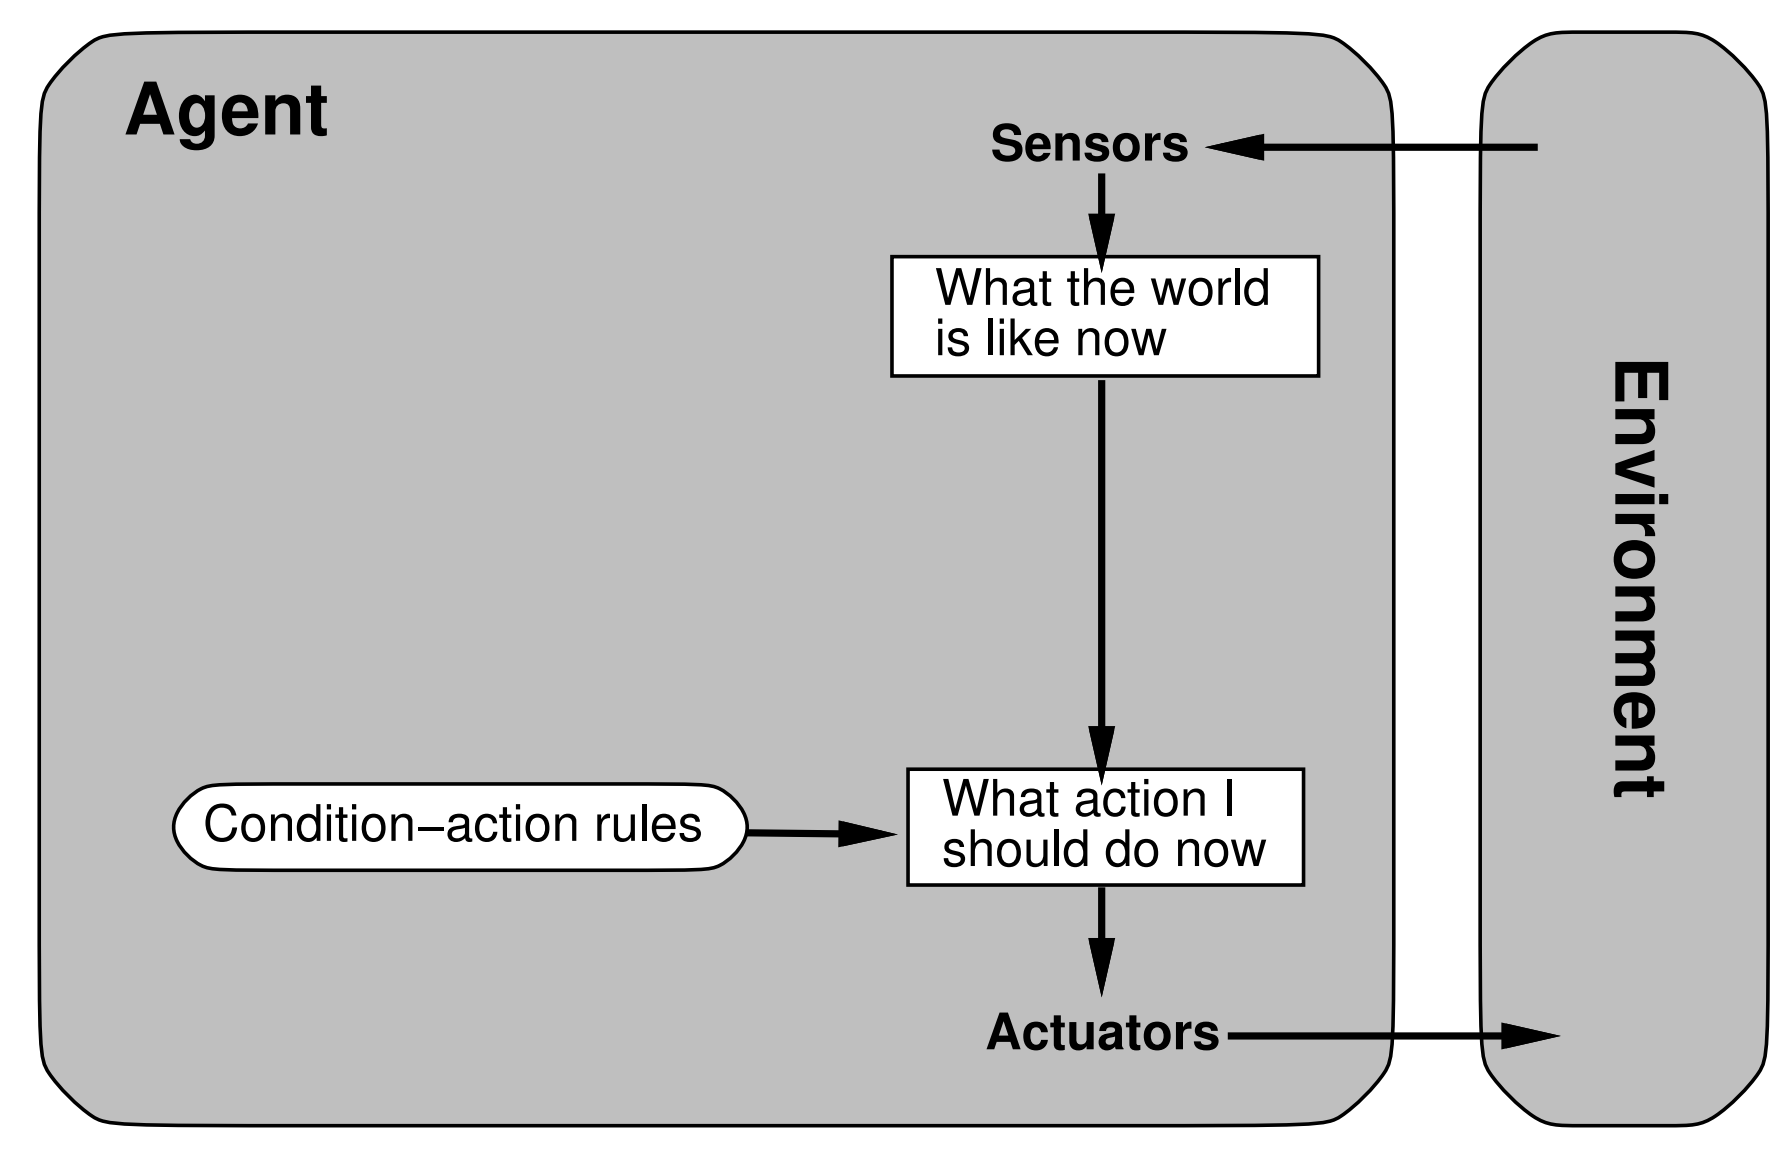
\includegraphics[width=0.4\textwidth ]{images/reflexAgent.png}
    \caption{Reflex agent diagram}
\end{figure}\bigskip

A \textbf{Model-Based Reflex Agent} is an enhanced version of the previous one, the key enhancement here is the inclusion of an \textit{Internal State} and a \textit{Model of the World} to make up for the agent's limited view of the environment. The internal state cannot simply be the last thing the agent saw; it needs to be updated to reflect reality. This is done using a Model of the World, which contains two key pieces of knowledge:\begin{itemize}
    \item 
    How the world evolves independently of the agent, his accounts for changes in the environment that occur regardless of the agent's actions (e.g., a clock ticking, an external event).
    \item
    How the agent's own actions affect the world, this is the effect of the agent's previous action (e.g., if the agent drove forward, its position changed).
\end{itemize}

\begin{figure}[h!]
    \centering
    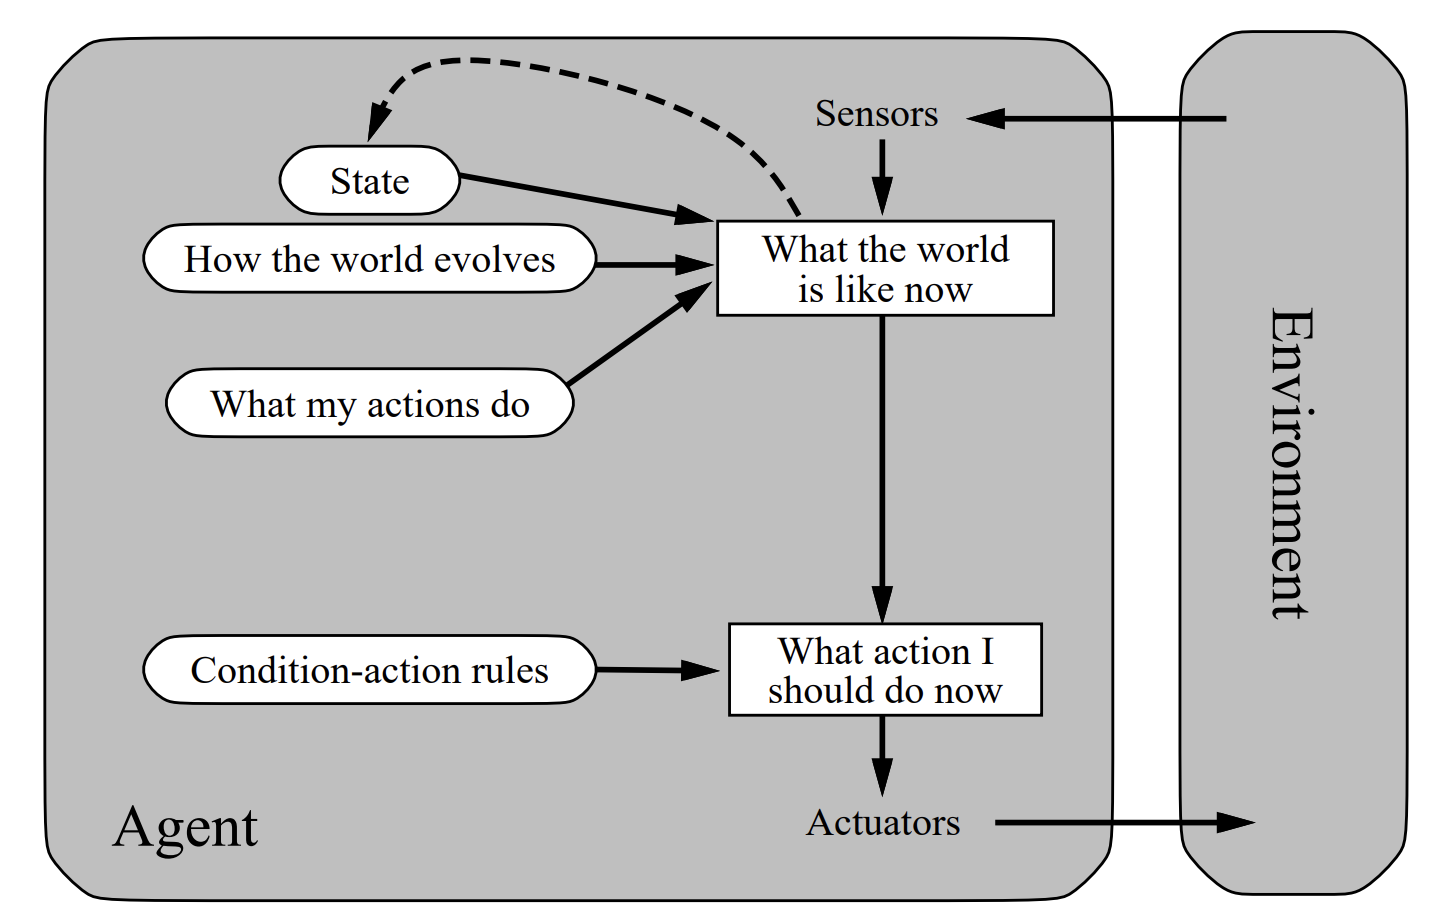
\includegraphics[width=0.4\textwidth ]{images/ModelreflexAgent.png}
    \caption{Model Based Reflex agent diagram}
\end{figure}\bigskip

If a model based reflex agent consider the future prospective, is a \textbf{Goal Based Agent}, as shown in figure \ref{img:goal_agent}.

\begin{figure}[h!]
    \centering
    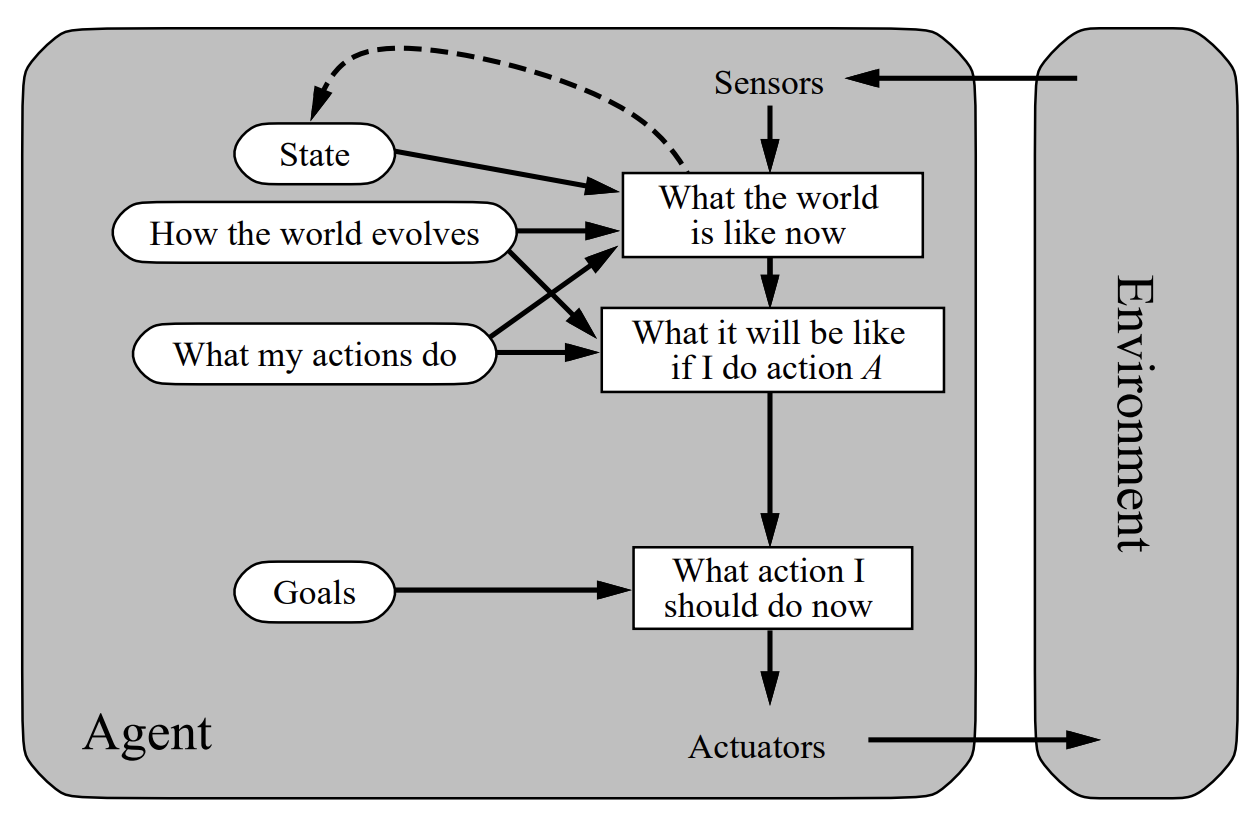
\includegraphics[width=0.4\textwidth ]{images/goal.png}
    \caption{Goal Based agent diagram}
    \label{img:goal_agent}
    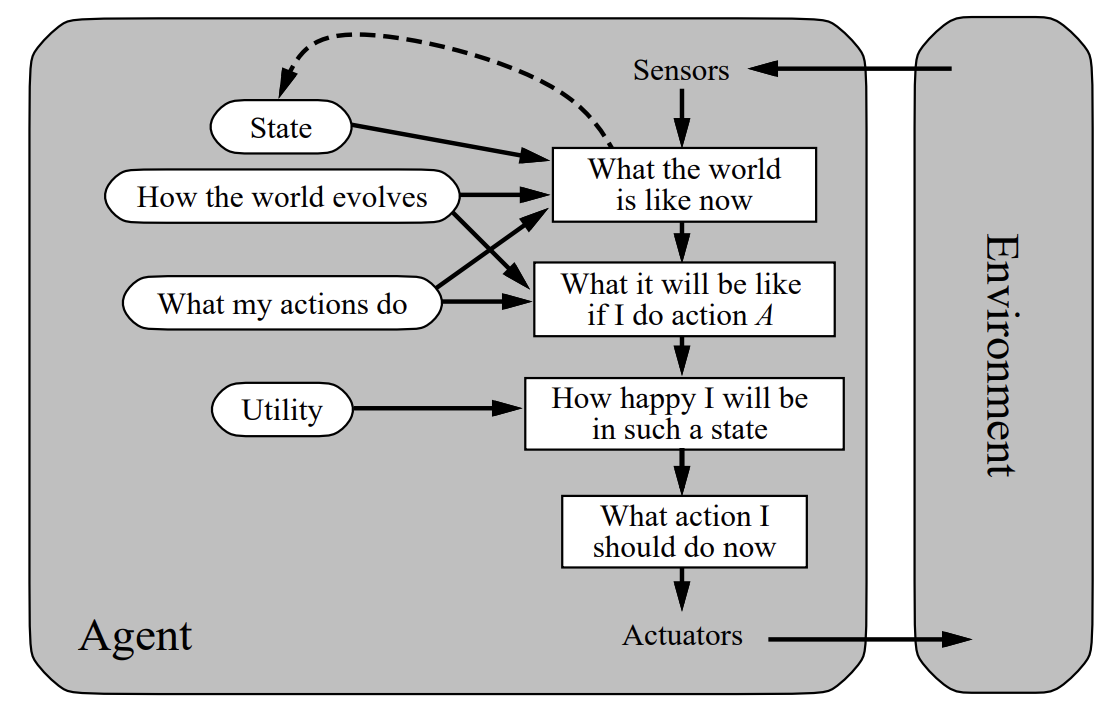
\includegraphics[width=0.4\textwidth ]{images/utility.png}
    \caption{Utility Based agent diagram}
\end{figure}\bigskip

A \textbf{Utility Based Agent} is equipped with a \textit{utility function} that maps a state to a number which represents how
desirable the state is. Agent’s utility function is an internalization of the performance function.\bigskip

A \textbf{Learning Agent} is an architecture designed to improve its efficiency over time by separating four functions:\begin{itemize}
    \item  the performance element selects actions\item  
     the critic provides feedback on those actions against a standard\item   the learning element uses this feedback to update the agent's internal knowledge\item   the problem generator suggests exploratory actions to gain new knowledge. This structure enables the agent to continuously adapt and improve its decision-making.
\end{itemize}

\begin{figure}[h!]
    \centering
    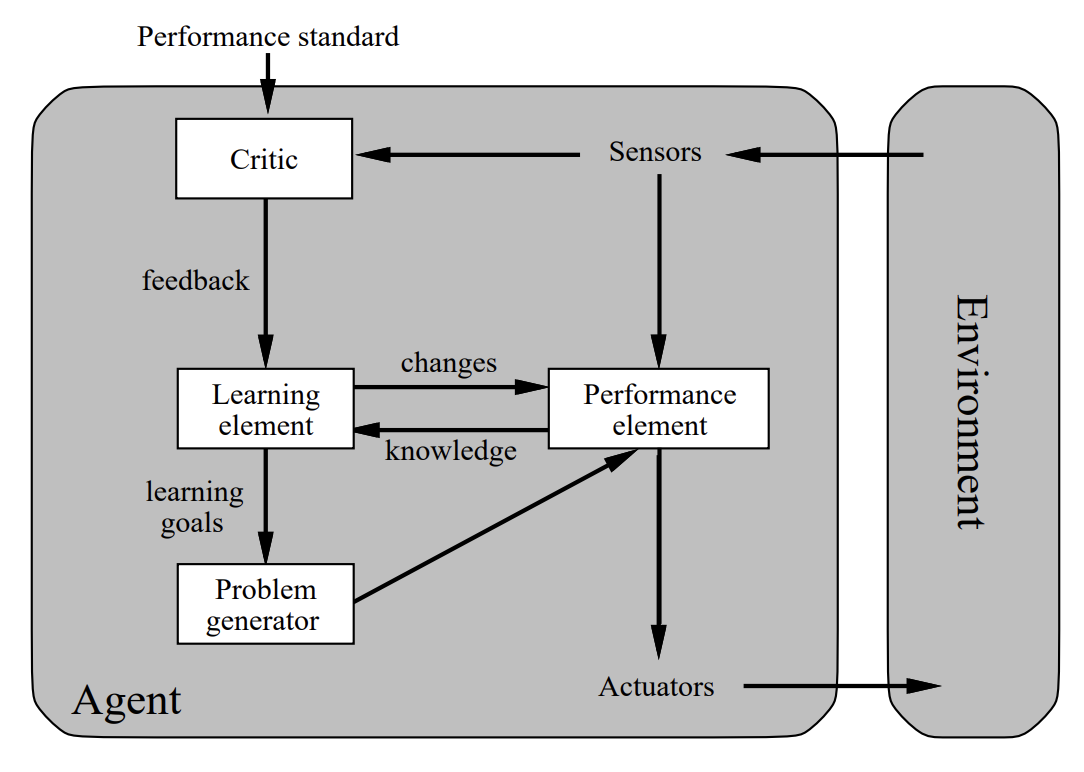
\includegraphics[width=0.4\textwidth ]{images/learn_agent.png}
    \caption{Learning agent diagram}
\end{figure}\bigskip

An agent can be classified in one of the following groups:\begin{itemize}
    \item a \textbf{domain specific agent }  is a solver specific to a particular problem (such as playing chess), is usually more efficient.
    \item a \textbf{general agent} is a solver for general problems, such as learning the rule of any board game, is usually more intelligent but less efficient.
\end{itemize}
\subsection{The Environment}
An environment can be classified in terms of different attributes:\begin{itemize}
    \item An environment can be \textbf{fully observable} if all the relevant information are accessible to the sensors, otherwise is \textbf{partially observable}.
    \item If there are no uncertainty, the environment is \textbf{deterministic}. An environment is \textbf{stochastic} if uncertainty is quantified by using probabilities, otherwise is \textbf{non deterministic} if uncertainty is managed as actions with multiple outcomes.
    \item An environment is \textbf{episodic} if the correctness of an action can be evaluated instantly, otherwise if are evaluated in the future developments, is \textbf{sequential}. 
    \item An environment can be \textbf{static} or \textbf{dynamic}, if itdoes not change, but the agent's performance
score changes, the environment is called \textbf{semi-dynamic}.
    \item An environment can be perceived as \textbf{discrete} or \textbf{continuous}.
    \item In a single environment there may be multiple agent, that can be \textbf{competitive} or \textbf{cooperative}.
\end{itemize}
Many sub-areas of AI can be classified by:\begin{itemize}
    \item Domain-specific vs. general.
    \item The environment.
    \item Particular agent architectures sometimes also play a role, especially
    in Robotics.
\end{itemize}
It follows a classification of some areas in terms of the attributes we discussed:\begin{itemize}
    \item \textbf{Classical Search}, the environment is\begin{itemize}
        \item fully observable
        \item deterministic
        \item static 
        \item sequential
        \item discrete
        \item single-agent
    \end{itemize}
    and the approach is \textit{domain specific}.
    \item \textbf{Planning}, the environment is\begin{itemize}
        \item fully observable
        \item deterministic
        \item static
        \item sequential 
        \item discrete
        \item single-agent
    \end{itemize}
    and the approach is \textit{general}.
    \item \textbf{Adversarial Search}, the environment is\begin{itemize}
        \item fully observable
        \item deterministic
        \item static 
        \item sequential    
        \item discrete
        \item multi-agent
    \end{itemize}
    and the approach is \textit{domain specific}.
    \item \textbf{General Game Playing}, the environment is\begin{itemize}
        \item fully observable
        \item deterministic
        \item static 
        \item sequential    
        \item discrete
        \item multi-agent
    \end{itemize}
    and the approach is \textit{general}.
    \item \textbf{Constraint Satisfaction \& Reasoning}, the environment is\begin{itemize}
        \item fully observable
        \item deterministic
        \item static 
        \item episodic    
        \item discrete
        \item single-agent
    \end{itemize}
    and the approach is \textit{general}.
    \item \textbf{Probabilistic Reasoning}, the environment is\begin{itemize}
        \item partially observable
        \item stochastic
        \item static 
        \item episodic    
        \item discrete
        \item single-agent
    \end{itemize}
    and the approach is \textit{general}.
\end{itemize}
\chapter{Search Problems}
\section{Classical Search}
Let's consider two basic example of classical search problems, the first one is the following:\begin{center}
    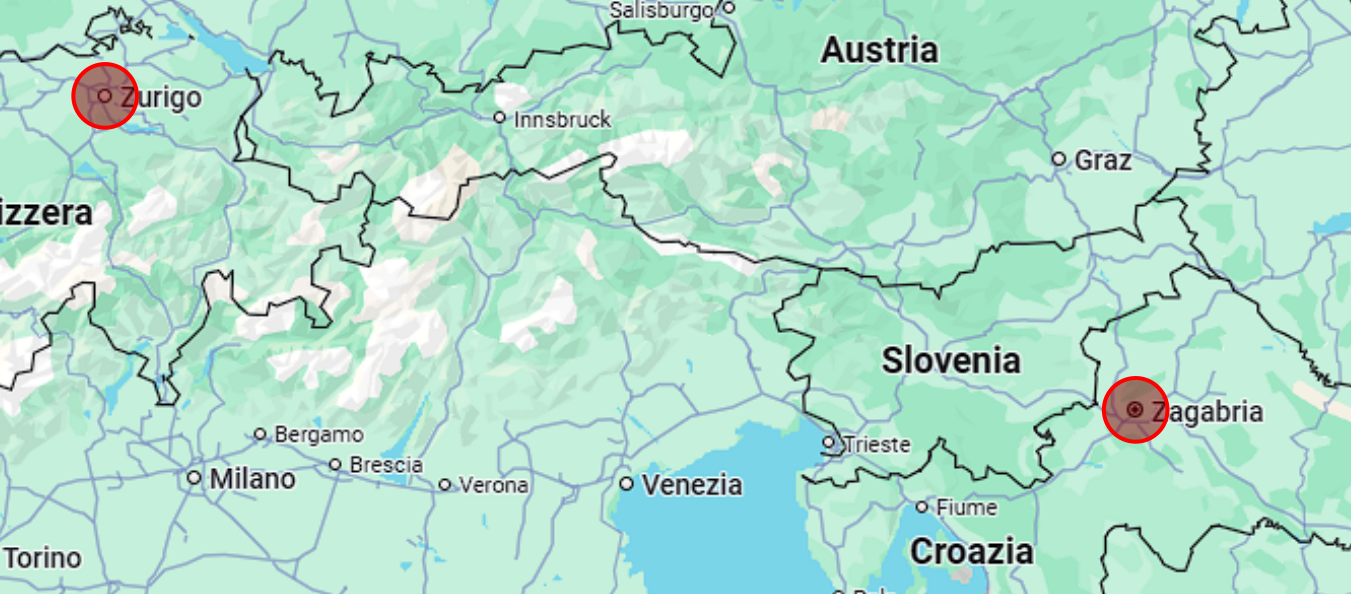
\includegraphics[width=0.5\textwidth ]{images/map_search.png}
\end{center}
Starting from Zurigo, we would like to find a route to Zagabria. We have an initial state (Zurigo), and we have to apply actions (drive) to reach the goal state (Zagabria). Another example is the following, we want to solve the tiles-puzzle game, shown in figure \ref{img:tiles}, to reach the left state, starting from the right one, the actions to perform is the move of the tiles. A performance measure could be to minimize the summed-up action costs.

\begin{figure}[h!]
    \centering
    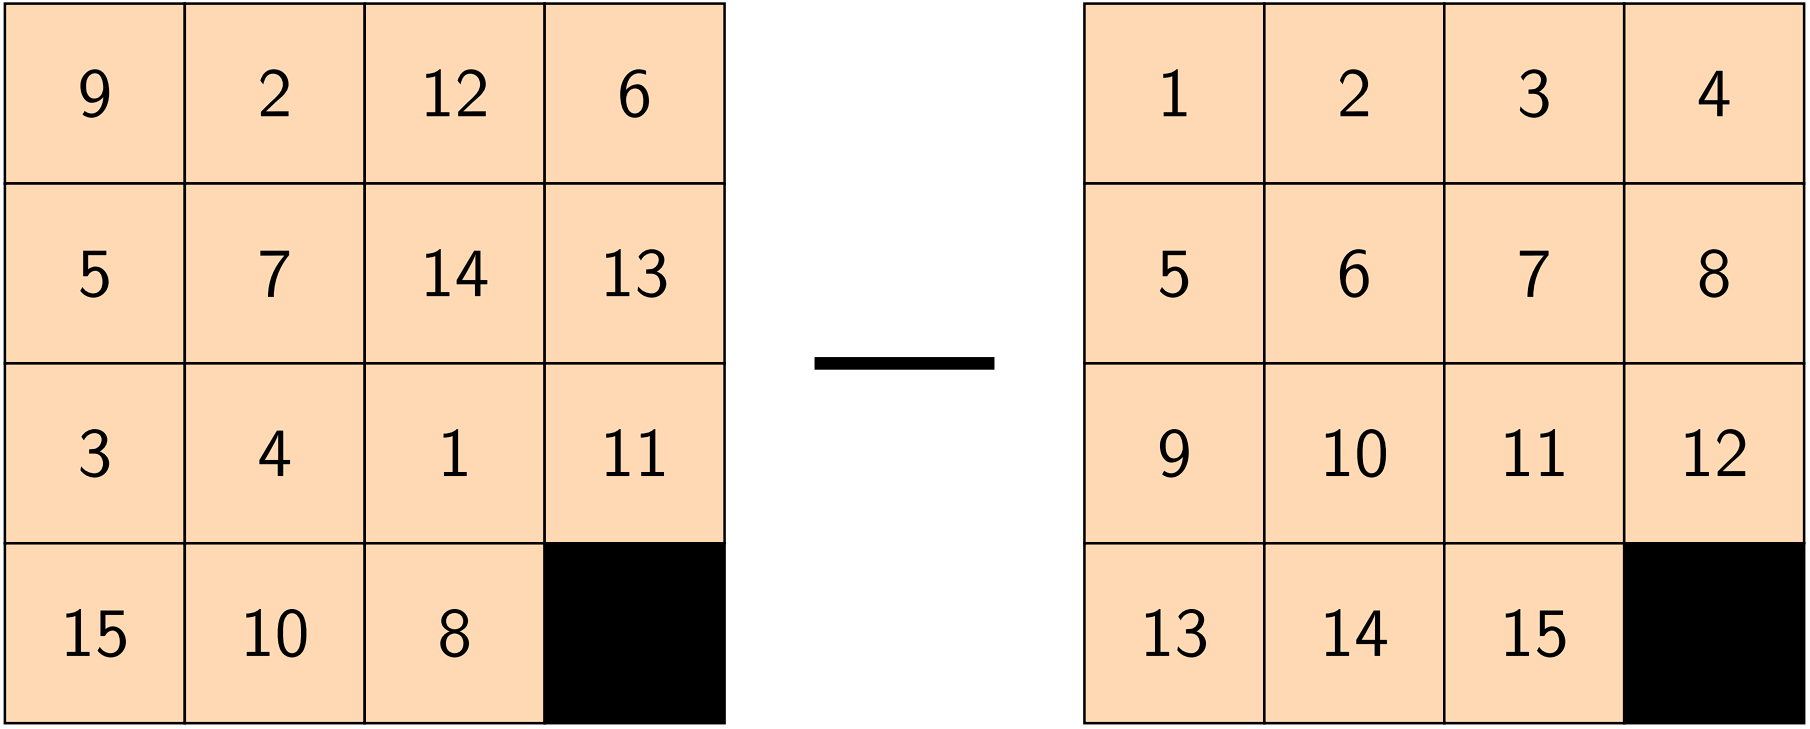
\includegraphics[width=0.6\textwidth ]{images/tile.png}
    \caption{The tile game}
    \label{img:tiles}
\end{figure}

In the classical search context, we restrict the agent's environment to a very simple setting, with a finite number of states and actions, a single agent, a fully observable stati environment that doesn't evolve, given that assumption, the classical search problems are the simplest one, despite that, are very important problems in practice.\bigskip

\noindent Every problem specifies a state space.

\begin{definition}
    A \textbf{State Space} is a 6-tuple $\Theta=(S,A,c,T,I,S^G)$ where:\begin{itemize}
        \item $S$ is a finite set of the \textit{states}.
        \item $A$ is a finite set of \textit{actions}.
        \item $c:A\rightarrow\R^+$ is the \textit{cost function}.
        \item $T\subseteq S\times A\times S $ is the \textit{transition relation}, that describes how an action on a given state make the agent evolve to the next state. We assume that the problem is deterministic, so for all $s\in S$, $a\in A$, if $(s,a,s')\in T$ and $(s,a,s'')\in T$ then $s'=s''$.
        \item $I\in S$ is the \textit{initial state}
        \item $S^G\subseteq S$ is the set of the \textit{goal states}, where we want to end.
    \end{itemize}
\end{definition}
A transition $(s,a,s')$ can be denoted $s \xrightarrow{a} s'$, we say that $s\rightarrow s'$ if $\exists a$ such that $(s,a,s')\in T$ . We say that $\Theta$ has \textit{unit costs} if $\forall a\in A, \ \ c(a)=1$. A state space can be illustrated as a directed labeled graph. \begin{definition}
    Let $\Theta=(S,A,c,T,I,S^G)$ to be a state space, we say that\begin{itemize}
        \item $s'$ is a \textbf{successor} of $s$ if $s\rightarrow s'$
        \item $s'$ is a \textbf{predecessor} of $s$ if $s'\rightarrow sT$
        \item we say that $s'$ is \textbf{reachable from} $s$ if\begin{align}
            &\exists (a_1\dots, a_n)\subseteq A\\
            &\exists (s_2\dots, s_{n-1})\subseteq S\\
            &(s,a_1,s_2)\in T\\
            &(s_2,a_2,s_3)\in T\\
            \vdots \\
            &(s_{n-1},a_n,s')\in T 
        \end{align}
        we can write the sequence as follows\begin{equation}
            s\xrightarrow{a_1}s_2,\dots, s_{n-1}\xrightarrow{a_n}s'.
        \end{equation}
        \item We say that $s$ is \textbf{reachable} (without reference state) if is reachable from $I$.
        \item $s$ is \textbf{solvable} if there exists $s'\in S^G$ such that $s'$ is reachable from $s$, otherwise $s$ is \textbf{dead end}.
    \end{itemize}
\end{definition}
\begin{definition}
    Let $\Theta=(S,A,c,T,I,S^G)$ to be a state space, and let $s\in S$. A \textbf{solution} for $s$ is a path from $s$ to some goal state $s'\in S^G$. The solution is \textbf{optimal} if it's cost is minimal, let $H$ to be the set of all possible solution (sequence of states) for $s$\begin{equation}
        H=\{\text{paths from }s\text{ to }s'\in S^G\}=\{(s_{i0},s_{i1},s_{i1},\dots s_{in})  : s_{in}\in S^G, \ s_{i0}=s\}
    \end{equation}
    where $n^i$ is the length of the $i$-th solution.
    The optimal solution is\begin{equation}
        \arg \min_{(s,s_{i1},\dots s_{in})\in H}\sum_{j=0}^{n^i} c(s_{ij}).
    \end{equation}
\end{definition}
A solution for $I$ is called \textbf{solution for $\Theta$}, if such that solution exists, $\Theta$ is \textbf{solvable}.
\subsection{Vacuum Cleaner Example}
Let's consider a vacuum cleaner, that is the agent of our problem, the goal is to clean a room, the vacuum cleaner can be in two possible points (left and right), this points can be clean or dirty. The agent can perform the following actions\begin{itemize}
    \item move right 
    \item move left 
    \item suck the dust on the floor
\end{itemize}
there are 8 possible states\begin{itemize}
    \item left point clean, right point clean, vacuum cleaner is on right point
    \item left point dirty, right point clean, vacuum cleaner is on right point
    \item left point clean, right point dirty, vacuum cleaner is on right point
    \item left point dirty, right point dirty, vacuum cleaner is on right point
    \item left point clean, right point clean, vacuum cleaner is on left point
    \item left point dirty, right point clean, vacuum cleaner is on left point
    \item left point clean, right point dirty, vacuum cleaner is on left point
    \item left point dirty, right point dirty, vacuum cleaner is on left point
\end{itemize}
the initial state is the one with the left point dirty, right point dirty, and the vacuum cleaner on the left point, we denote the actions $R$ (move right), $L$ (move left), $S$ suck. The state space of the problem is show in figure \ref{img:vacuum_cleaner}. 

\begin{figure}[h!]
    \centering
    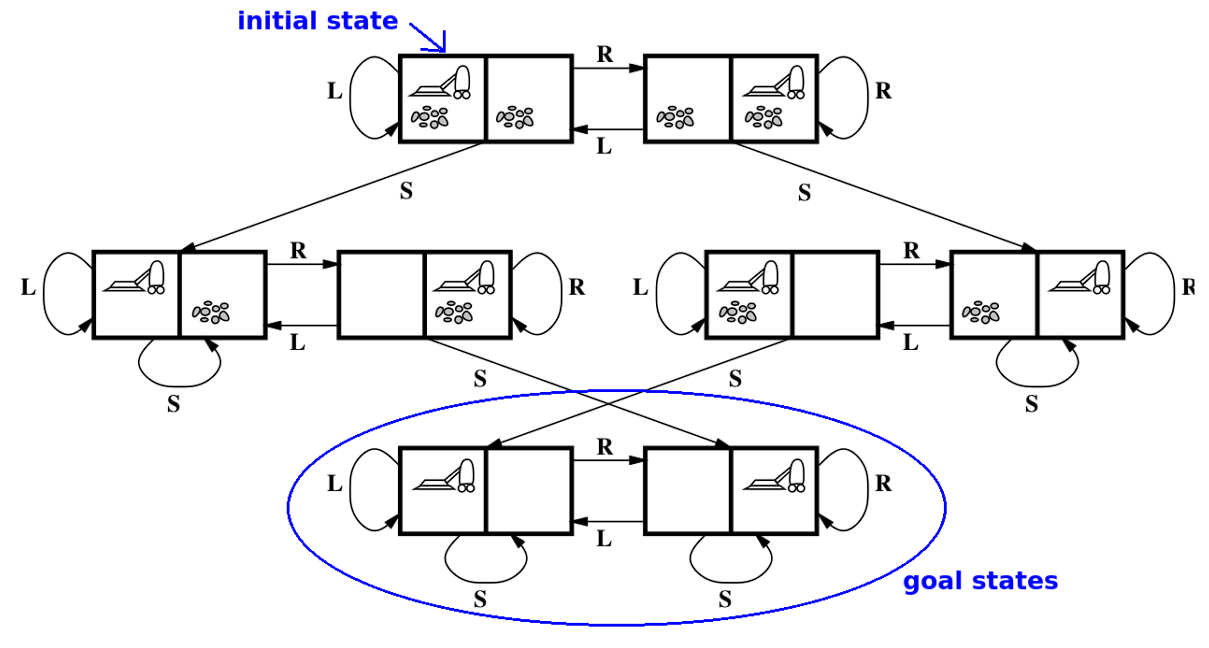
\includegraphics[width=0.6\textwidth ]{images/vacuum.png}
    \caption{The vacuum cleaner state space}
    \label{img:vacuum_cleaner}
\end{figure}
Some example of set of actions that can lead from the initial state to a goal state are\begin{align*}
    &S\longrightarrow R\longrightarrow S\\
    &S\longrightarrow R\longrightarrow R\longrightarrow S\\
    &R\longrightarrow S\longrightarrow L\longrightarrow S
\end{align*}

Typically, the state space is exponentially large in the size of its specification, search problems are typically computationally hard and/or $\mathsf{NP}$-complete. We say that we can give an \textit{explicit description} of a search problem if we can define his state space as a graph.
\section{Problem Descriptions}
\begin{definition}
    We have a \textbf{black box description} of the problem if we can't describe the state space explicitly but we can\begin{itemize}
        \item Know which is the initial state
        \item Check if a given state is a goal state
        \item Check the cost of a given action $a$
        \item Given a state $s$, check all the actions that are applicable to state $s$
        \item Given a state $s$ and an applicable action $a$, we can get the successor state.
    \end{itemize}
\end{definition}
We can think about it in a programming-way, given a problem described by $\Theta=(S,A,c,T,I,S^G)$, we can't check directly $\Theta$, but we have an \textit{API} of the problem that provide the following functions \begin{itemize}
    \item \texttt{InitialState()} : return the initial state of the problem
    \item \texttt{GoalTest($s$)} : return true if and only if $s\in S^G$
    \item \texttt{Cost}($a$ : return $c(a)$)
    \item \texttt{Actions}($s$) : return the set $\{ a \ : \ \exists  s\xrightarrow{a} s'\in T \text{ for some }s'\in S\}$
    \item \texttt{ChildState}($s,a$) : return $s'$ if $s\xrightarrow{a} s'\in T$.
\end{itemize}
We \textbf{specify} a search problem if we can program/access to such an \textit{API}. There are a declarative description too.
\begin{definition}
\end{definition}
We have a \textbf{declarative description} of the problem if is described by the following sets:\begin{itemize}
    \item $P$ is a set of boolean variables (\textit{propositions})
    \item $I\subseteq P$ is the subset of $P$ indicating which propositions are true in the initial states.
    \item $G\subset P$ is the subset of $P$ describing the goal states in the following way\begin{itemize}
        \item a state $s$ is a set of propositions 
        \item $s\subseteq G \iff s$ is a goal state
    \end{itemize}
    \item $A$ is a set of actions, each action $a$ is described by\begin{itemize}
        \item a set $pre_a\subseteq P$ of \textit{precondition}, $a$ can be performed if and only if the conditions in $pre_a$ are true.
        \item a set of propositions $add_a$
        \item a set of propositions $del_a$
        \item the outcome of each action is the state $(\{s\}\cup add_a )\backslash del_a$
        \item $c:A\rightarrow\R$ is the cost function.
    \end{itemize}
\end{itemize}
Declarative descriptions are strictly more powerful than black box ones. In this section we assume the black box description. In principle, the search strategies we will discuss can be used with any
problem description that allows to implement the black box \textit{API}.
\subsection{Missionaries and Cannibals Example}
The problem is the following\begin{itemize}
    \item there are a river and a boat that can carry the people from the left bank to the right 
    \item there are 6 people, 3 missionaries and 3 cannibals 
    \item the boat can carry 0, 1 or 2 people at the same time, not 3 
    \item the goal is to get  everybody to the left bank
    \item if at any time, there are more cannibals than missionaries in one bank, the missionaries get killed and the game is lost. 
\end{itemize}
We can model the problem as follows\begin{itemize}
    \item the state space $S$ is \begin{equation}
        S=\{(M,C,B) \ : \ M+C=6, \ 0\le M \le 3, \ 0\le C \le 3, \  B\in\{0,1\}\}
    \end{equation}
    $M$ represents the current number of missionaries on the right bank, $S$ represents the current number of cannibals on the right bank, $B=1$ if the boat is on the right bank, otherwise is on the left.
    \item the initial state is $(3,3,1)$
    \item the goal states are $S^G={(0,0,0),(0,0,1)}$
    \item each actions have the same cost, is negligible
    \item the action that can be performed are the following\begin{itemize}
        \item if $B=1$, we can subtract (in total) 1 or 2 from $M$ or $C$ (or both), and set $B=0$.
        \item if $B=0$, we can add (in total) 1 or 2 from $M$ or $C$ (or both), and set $B=1$.
    \end{itemize}
    an action is applicable if and only if the following condition are satisfied after\begin{itemize}
        \item $M\ge C$ if $M>0$, this decode the facts that the cannibals can't be more or equals than the missionaries on the right bank if there are missionaries on the left bank
        \item if $M<3$ (some missionaries are on the left bank) then $(3-M)>(3-C)$ the missionaries on the left bank must be greater then the cannibals on the left bank.
    \end{itemize}
\end{itemize}
To search a solution we can start from the initial state and expand the tree of possible solutions accordingly to the applicable actions.\begin{center}
    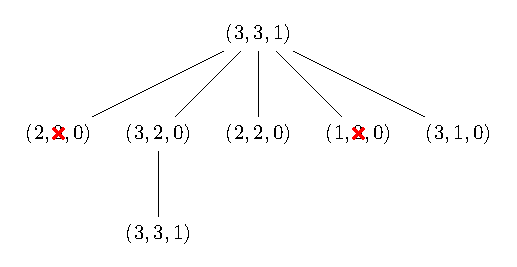
\includegraphics[width=0.5\textwidth ]{images/missionaries.eps}
\end{center}
\subsection{Tree and Graph Search}
In the search context the following terminology is used
\begin{itemize}
    \item Search node $n$: Contains a state reached by the search, plus information about how it was reached.
    \item Path cost $g(n)$: The cost of the path reaching $n$.
    \item Optimal cost $g^*$: The cost of an optimal solution path. For a state $s$, $g^*(s)$ is the cost of a cheapest path reaching $s$.
    \item Node expansion: Generating all successors of a node, by applying all actions applicable to the node's state $s$. Afterwards, the state $s$ itself is also said to be expanded.
    \item Search strategy: Method for deciding which node is expanded next.
    \item Open list: Set of all nodes that currently are candidates for expansion. Also called frontier.
    \item Closed list: Set of all states that were already expanded. Used only in graph search, not in tree search (up next). Also called explored set.
\end{itemize}
When we explore the state space of a problem we can maintain a closed list of all the node that has been already searched, to check for each generated new node if is already in the list (if so, we discard it). If such list is used, the search is called \textbf{graph search}, else, if the same state may appear in many search nodes, is called \textbf{tree search}. The tree search doesn't use a list so require less memory.\bigskip

When we analyze a search algorithm, we are interested in various properties\begin{itemize}
    \item \textbf{Completeness}: the algorithm is guaranteed to find a solution (it there are one).
    \item \textbf{Optimality}: the returned solution is guaranteed to be optimal. 
    \item \textbf{Time Complexity}: How long does it take to find a solution? (Measured
in generated states).
    \item \textbf{Space Complexity}: How much memory does the search require?
(Measured in states).
    \item \textbf{Branching Factor}: The number $b$ of how many successor a state may have.
    \item \textbf{Gal depth}: the number $d$ of action required to reach the shallowest (nearest to the initial state) goal state.
\end{itemize}
\section{Blind Search}
We talk about \textit{blind search} if the problem does not require any input beyond the problem API. Does not require any additional work from the programmer. For each node $n$ in the search context, we define the following data structure:\begin{itemize}
    \item $n$.State is the state which te node contains 
    \item $n$.Parent is node in the search tree that generated this node
    \item $n$.Action is the action that was applied to the parent to generate the node
    \item $n$.PathCost, also denoted $g(n)$, is the cost of the path from the initial state to the node (as indicated by the parent pointers).
\end{itemize}
On a node we can perform the following operations\begin{itemize}
    \item Solution($n$) returns the path from the initials state to $n$
    \item ChildNode($n,a$) returns the node $n$ corresponding to the application of action $a$ in state $n$.State. 
\end{itemize}
We also have the open list (called frontier) where we can perform the following actions:\begin{itemize}
    \item Empty?(frontier) returns true if and only if there are no more elements in the
open list.
    \item Pop(frontier) returns the first element of the open list, and
removes that element from the list.
    \item Insert(element,frontier) inserts an element into the open list.
\end{itemize}
The insert function can put the element in front, in the last positions, or in other positions, it depends from the implementation (different implementations yield different search strategies).
\subsection{Breadth-First Search}
The strategy is to expand nodes in the order they were produced, as a FIFO queue, we expand the shallowest unexpanded node.
\begin{center}
    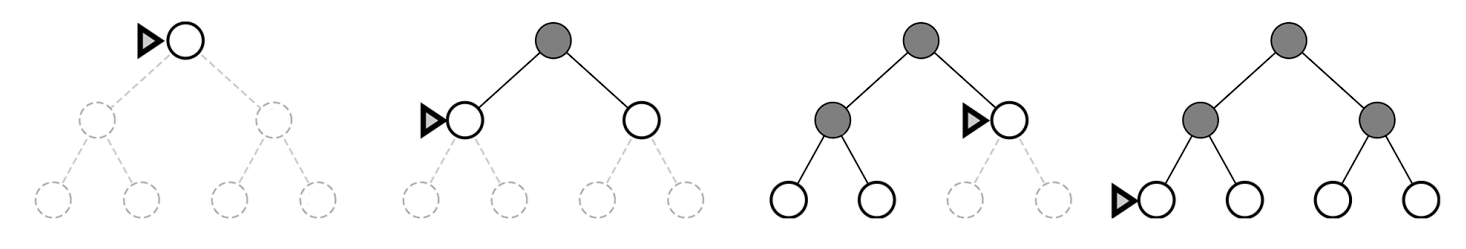
\includegraphics[width=1\textwidth ]{images/bfs.png}
\end{center}
This algorithm \ref{alg:BFS} is complete and optimal (in case of unit cost function). We are using the black box \textit{API}.

\begin{algorithm}
    \caption{Breadth-First Search}\label{alg:BFS}
    \begin{algorithmic}
    \Require $problem$
    \State $node\leftarrow$\texttt{InitialState()}
    \If{\texttt{GoalTest($node$.State)}}
    \State\Return Solution($node$)
    \EndIf
    \State $frontier\leftarrow$ a FIFO queue with $node$ in it
    \State $explored\leftarrow$ an empty set
    \While{true}
    \If{Empty?($frontier$)}
    \State\Return Failure
    \EndIf
    \State $node\leftarrow$pop($frontier$)
    \State add $node$.State in $explored$
    \For{each $action$ in \texttt{Actions($node$.State)}}
    \State $child\leftarrow$ChildNode($node,action$)
    \If{$child$.State is not in $explored$ or $frontier$}
    \If{\texttt{GoalTest($child$.State)}}
    \State\Return Solution($child$)
    \EndIf
    \State $frontier\leftarrow$Insert($child$,$frontier$)
    \EndIf
    \EndFor
    \EndWhile
    \end{algorithmic}
\end{algorithm}
Let $b$ to be the maximum branching factor and $d$ the depth of the shallowest goal state, an upper bound (in the worst case) for the number of nodes generated (time complexity) is\begin{equation}
    b+b^2+b^3\dots +b^d\in O(b^d)
\end{equation}
the same for the space complexity since  all generated nodes are kept in memory. Let's see an example, assume that $b=10$, the agent can generate $10^4$ nodes per second, and each node has a size of $1$ kilobyte, we have the following data:\begin{center}
    \begin{tabular}{|c|c|c|c|}
        \hline
        \textbf{Depth} & \textbf{Nodes} & \textbf{Time} & \textbf{Memory} \\
        \hline
        2 & 110 & 0.11 milliseconds & 107 kilobytes \\
        \hline
        4 & 11,110 & 11 milliseconds & 10.6 megabytes \\
        \hline
        6 & $10^6$ & 1.1 seconds & 1 gigabyte \\
        \hline
        8 & $10^8$ & 2 minutes & 103 gigabytes \\
        \hline
        10 & $10^{10}$ & 3 hours & 10 terabytes \\
        \hline
        12 & $10^{12}$ & 13 days & 1 petabyte \\
        \hline
        14 & $10^{14}$ & 3.5 years & 99 petabytes \\
        \hline
    \end{tabular}
\end{center}
The critical resource for this method is the memory.
\subsection{Depth-First Search}
The strategy is to expand the most recent explored node, as a LIFO queue, we expand the deepest unexpanded node. 
\begin{center}
    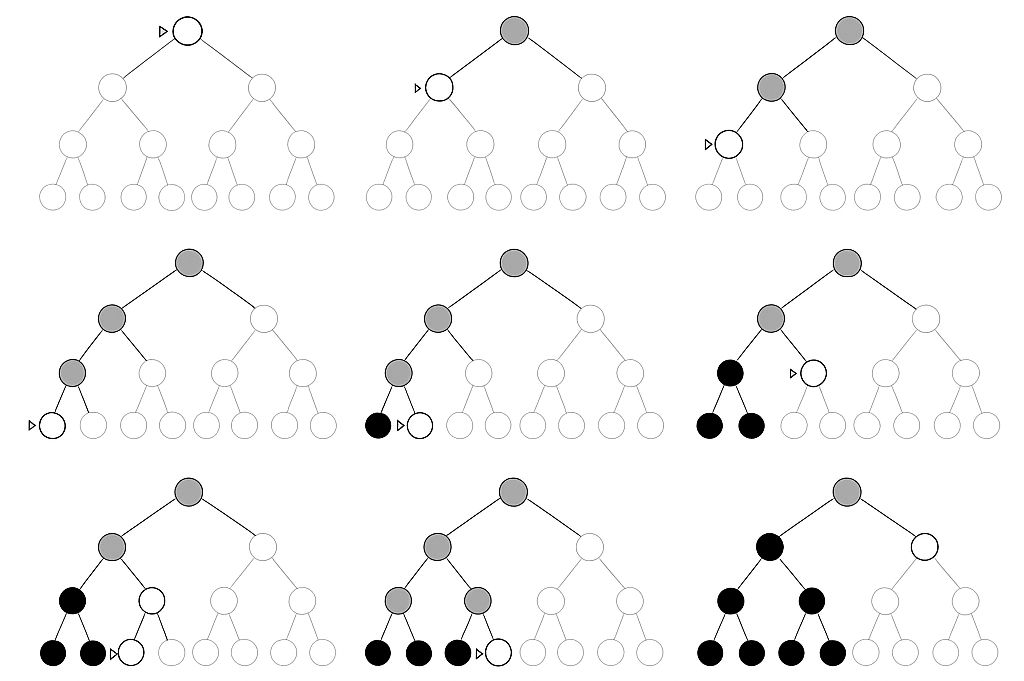
\includegraphics[width=0.7\textwidth ]{images/dfs.png}
\end{center}
The algorithm is not complete since it may take infinite time, since there is no check for cycles along the branches. It's not optimal since he chooses a direction and looks for a path to a goal state. Is typically implemented as a recursive function, as in algorithm \ref{alg:DFS}.\bigskip

\begin{algorithm}
    \caption{Depth-First Search}\label{alg:DFS}
    \begin{algorithmic}
    \Require $problem$, a node $n$
    \If{\texttt{GoalTest}($n$.\texttt{State})}
    \State\Return empty action sequence
    \EndIf
    \For{each $action$ in \texttt{Actions}($node$.\texttt{State})}
    \State $n'\leftarrow$ChildNode($node$,$action$)
    \State result$\leftarrow$Depth-First Search($problem$,$n'$)
    \If{result$\ne$ failure}
    \State\Return $action \ \circ$ result
    \EndIf
    \EndFor
    \State\Return failure
    \end{algorithmic}
\end{algorithm}

\noindent With $action \ \circ$ result is denoted the concatenation of actions. 
About the space complexity, this methods stores only a single path of actions, from the root to a leaf node, since once a
 node has been expanded, it can be removed from memory as soon as all its
 descendants have been fully explored.

 If $m$ is the maximal depth reached, the space occupied is in $O(bm)$. About the time complexity, in the worst case the nodes generated is in $O(b^m)$.
 \subsection{Uniform-Cost Search}
 This methods is equivalent to the well known Dijkstra's algorithm. We expand the node with the lowest path cost $g(n)$, the frontier is ordered by the path cost, with the lowest first. It differs from the BFS since a test is added to check if a better path is found to a node currently
 on the frontier.

 \begin{algorithm}
    \caption{Uniform-Cost Search}\label{alg:DFS}
    \begin{algorithmic}
    \Require $problem$
    \State $node\leftarrow$\texttt{InitialState()}
    \State $frontier\leftarrow$ priority queue ordered by ascending $g$
    \State $explored\leftarrow$ empty set of states
    \While{true}
    \If{Empty?($frontier$)}
    \State\Return failure 
    \EndIf
    \State $n\leftarrow$Pop($frontier$)
    \If{\texttt{GoalTest}($n$.State)}
    \State\Return Solution($n$)
    \EndIf
    $explored\leftarrow explored\cup n$.State
    \For{each $action$ in \texttt{Actions}($node$.\texttt{State})}
    \State $n'\leftarrow${ChildNode}($n$,$a$)
    \If{$n'$.State$\notin explored\cup$States($frontier$)}
    \State $frontier\leftarrow$insert($n'$,$frontier$)
    \Else{ \textbf{if} $\exists n''\in frontier \ : \ n''.$State=$n'$.State$ \land \ g(n')<g(n'')$}
    \State replace $n''$ with $n'$ in $frontier$
    \EndIf
    \EndFor
    \EndWhile
    \end{algorithmic}
\end{algorithm}
\begin{theorem}
    The Uniform-Cost search algorithm is optimal, since the Dijkstra's algorithm is optimal, and Uniform-cost search is equivalent to Dijkstra's algorithm on the state space graph.and 
\end{theorem}

The algorithm is complete if we assume that, the costs are strictly positive and the state space is finite. The time and space complexity are\begin{equation}
    O(b^{1+\lfloor\nicefrac{g^*}{*}\rfloor})
\end{equation}where\begin{itemize}
    \item $g^*$ is the cost of an optimal solution 
    \item $\epsilon=\min c$ is the positive cost of the cheapest action, the minimum of the function $c$.
\end{itemize}
\subsection{Iterative Deepening Search}
This is an altered version of the Depth-First Search algorithm, where we define a predetermined depth limit, and apply the DFS in function of that limit, iteratively applying this by increasing the depth limit each time.
\begin{center}
    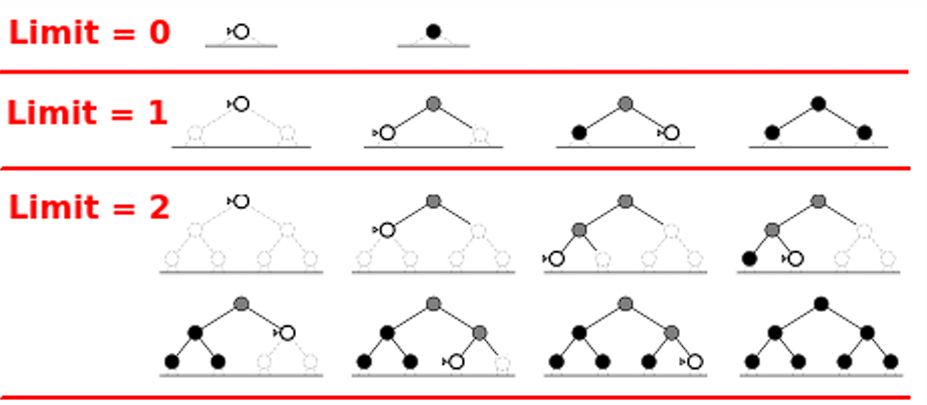
\includegraphics[width=0.7\textwidth ]{images/iterative_deep.png}
\end{center}
\end{document}